\documentclass[11pt]{article}
\usepackage{tikz}
%\usepackage{xfrac}
%\usepackage{hyperref}
%\usepackage[export]{adjustbox}
\def\checkmark{\tikz\fill[scale=0.4](0,.35) -- (.25,0) -- (1,.7) -- (.25,.15) -- cycle;} 
\usepackage{proj} 	% pull in style header
\usepackage{array}
\usepackage{sectsty}
\usepackage{soul}
\usepackage{float}
\usepackage{multirow} 
\usepackage{gensymb}
\restylefloat{table}

\lhead{ECE544: Embedded Systems on FPGAs}


%----------------------------------------------------------------------------------------
%	TITLE SECTION
%----------------------------------------------------------------------------------------


\newcommand{\horrule}[1]{\rule{\linewidth}{#1}} % Create horizontal rule command with 1 argument of height

\title{	
\normalfont \normalsize 
\textsc{\LARGE Portland State University}\\[1.5cm] % Name of your university/college
\textsc{\Large Embedded Systems on FPGAs}\\[0.5cm] % Major heading such as course name
\textsc{\large ECE544}\\[0.5cm] % Minor heading such as course title
%\textsc{Portland State University} \\ [25pt] % Your university, school and/or department name(s)
\horrule{1.2pt} \\[0.4cm] % Thin top horizontal rule
\huge Autonomous Robot Car \\ % The assignment title
\horrule{1.2pt} \\[0.5cm] % Thick bottom horizontal rule
}

%----------------------------------------------------------------------------------------
%	AUTHOR SECTION
%----------------------------------------------------------------------------------------


\begin{document}
\author{Erik Rhodes \and Caren Zgheib} % Your name
\maketitle % Print the title
\thispagestyle{empty}
\cfoot{\textit{Page \thepage { of} \pageref{LastPage}}}
\lhead{ECE544}
\chead{Final Project}
\rhead{Erik Rhodes \& Caren Zgheib}


\begin{figure}[h]\centering
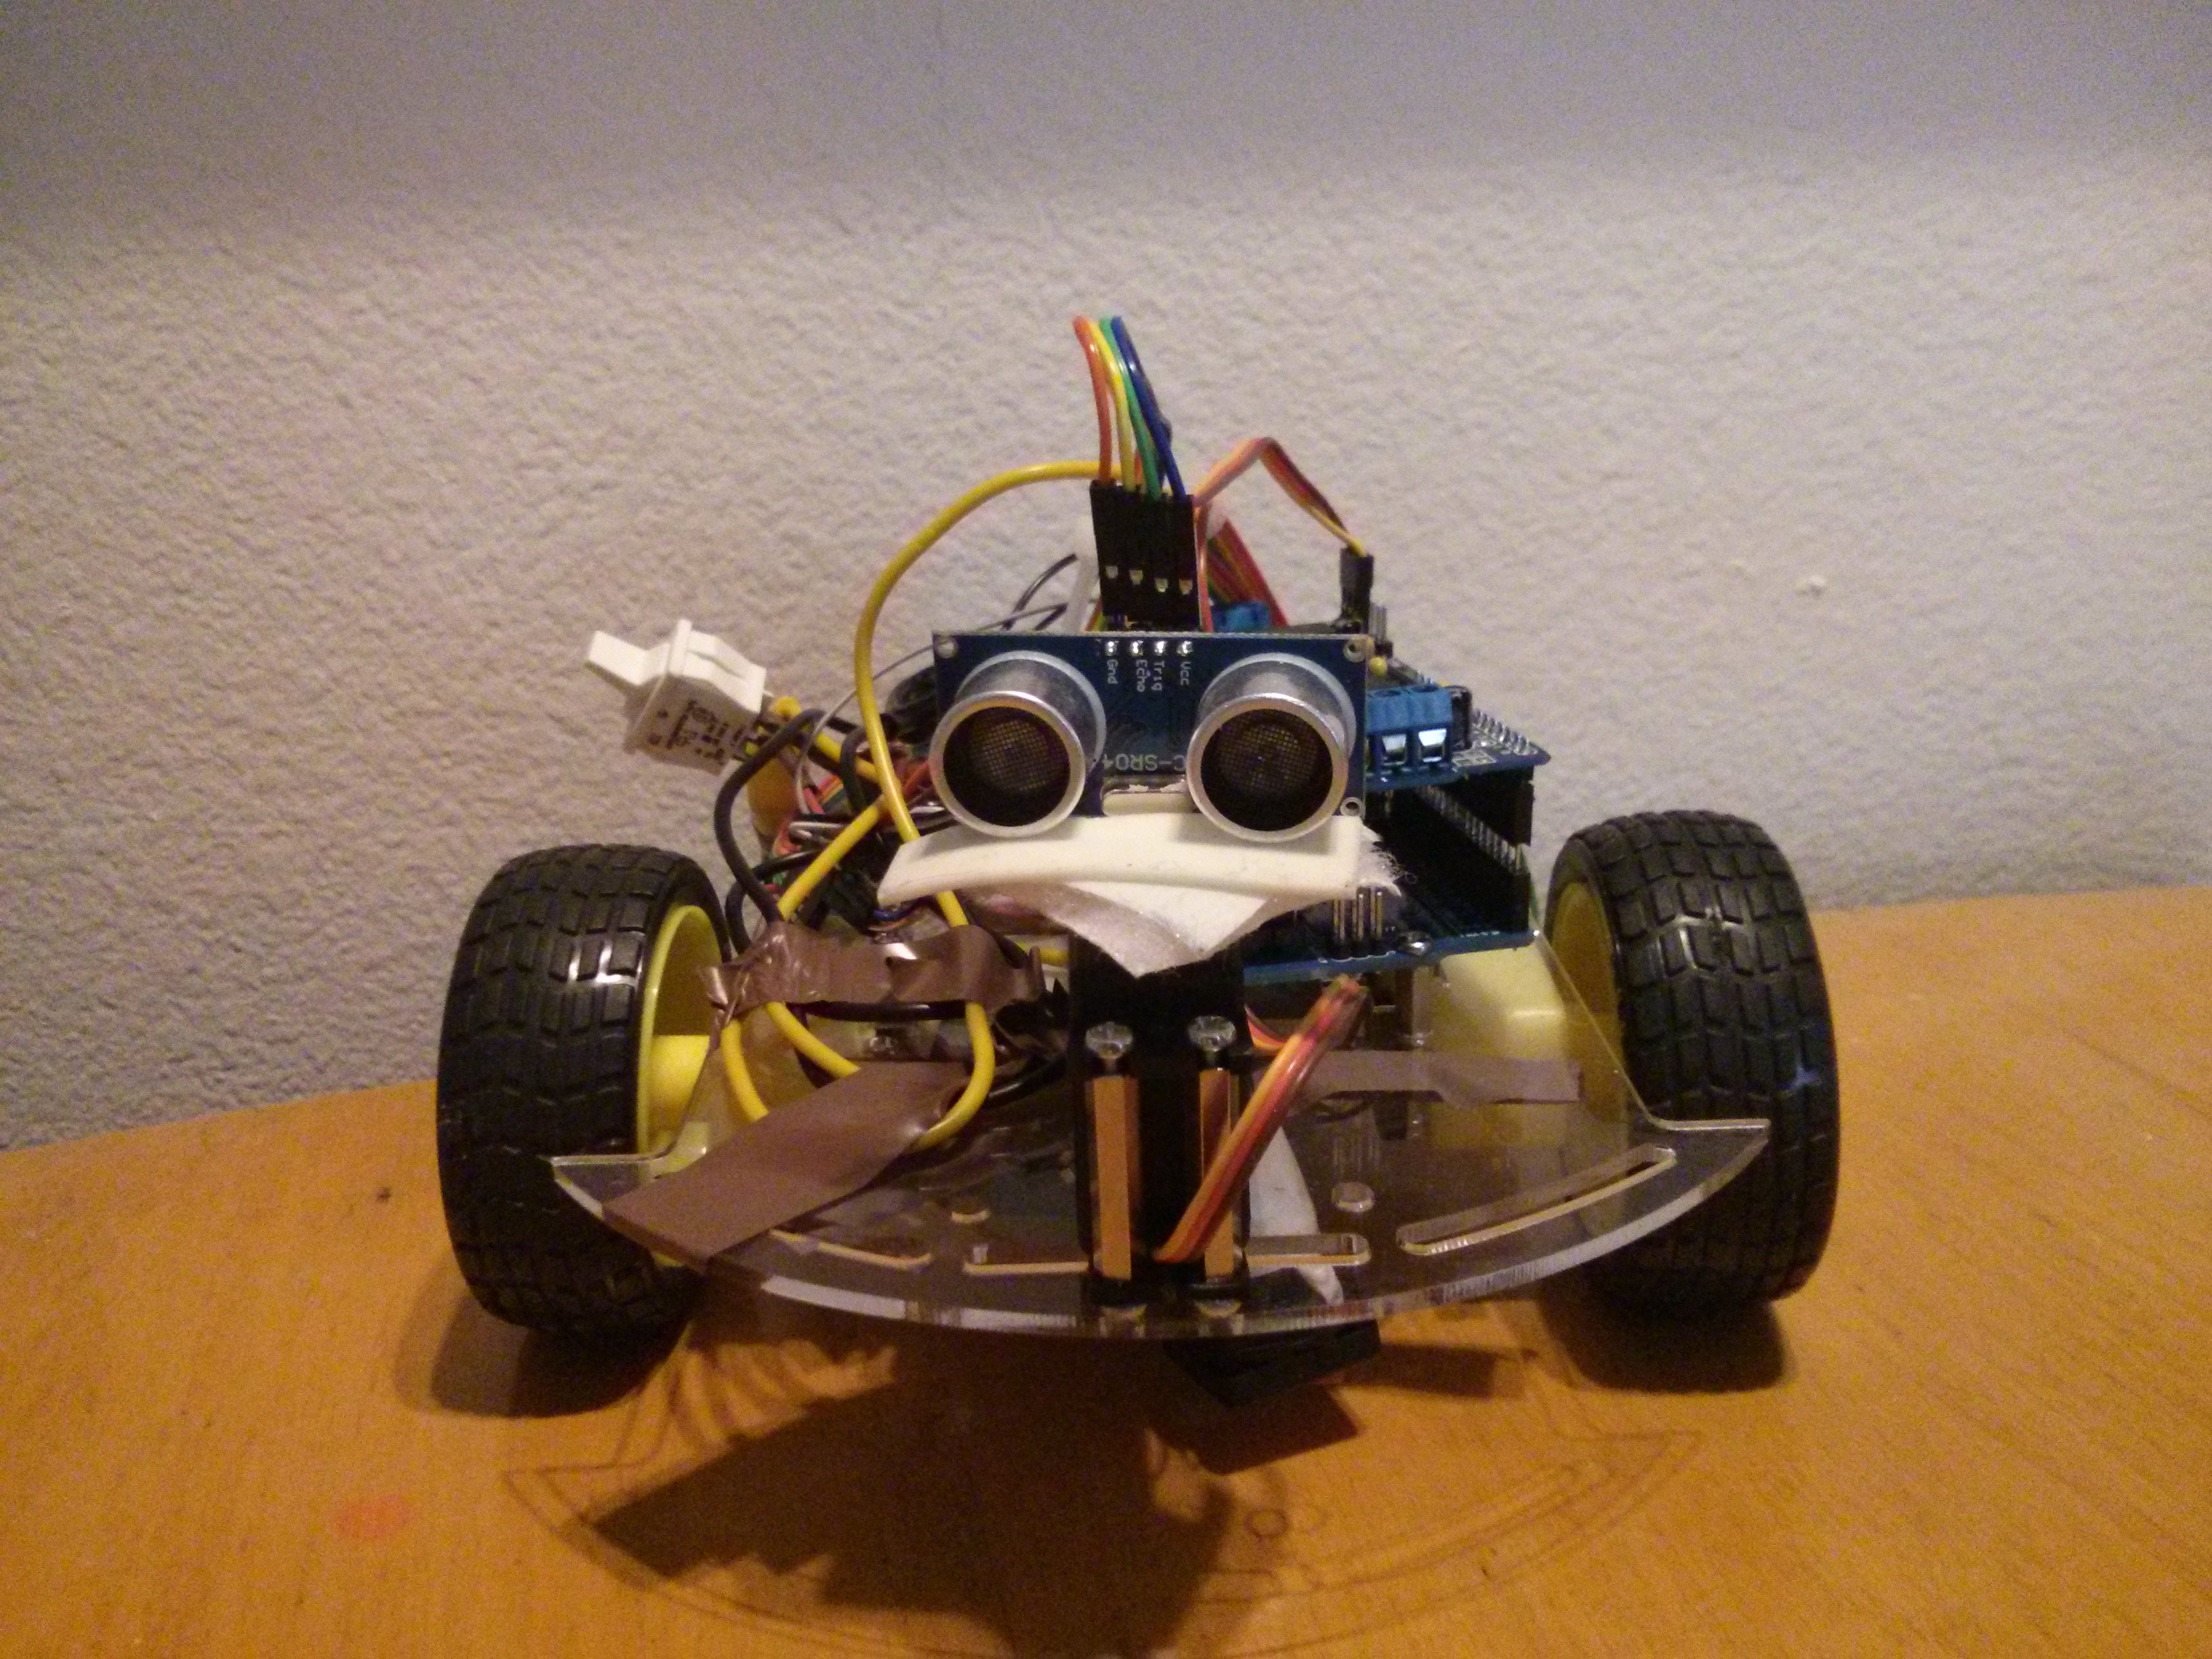
\includegraphics[height=0.65\textwidth]{images/bot_front.jpg}
		\label{bot_front}
	\end{figure}
	
\tableofcontents
\newpage

\section{Introduction} 
We created an autonomous robot car (SaMMY) that can successfully navigate its way through a given area without hitting any objects . It uses the popular \textbf{Arduino} platform and libraries along with a ultrasonic sensor for object detection. 

%TODO 
% Block diagram of arduino
% Other flowcharts?
% Explain algorithms

\section{Hardware Components}
%TODO References (oddwires)
There are many different components needed to successfully and robustly create an autonomous robot.  The bulk of our design used a robot kit we ordered online (ref).  We also added various parts to make the production time more convenient, including switches, additional batteries, and various cables.  The important components can be seen in Figure \ref{diagram} and are described in Table \ref{components}.


	\begin{figure}[h]\centering
	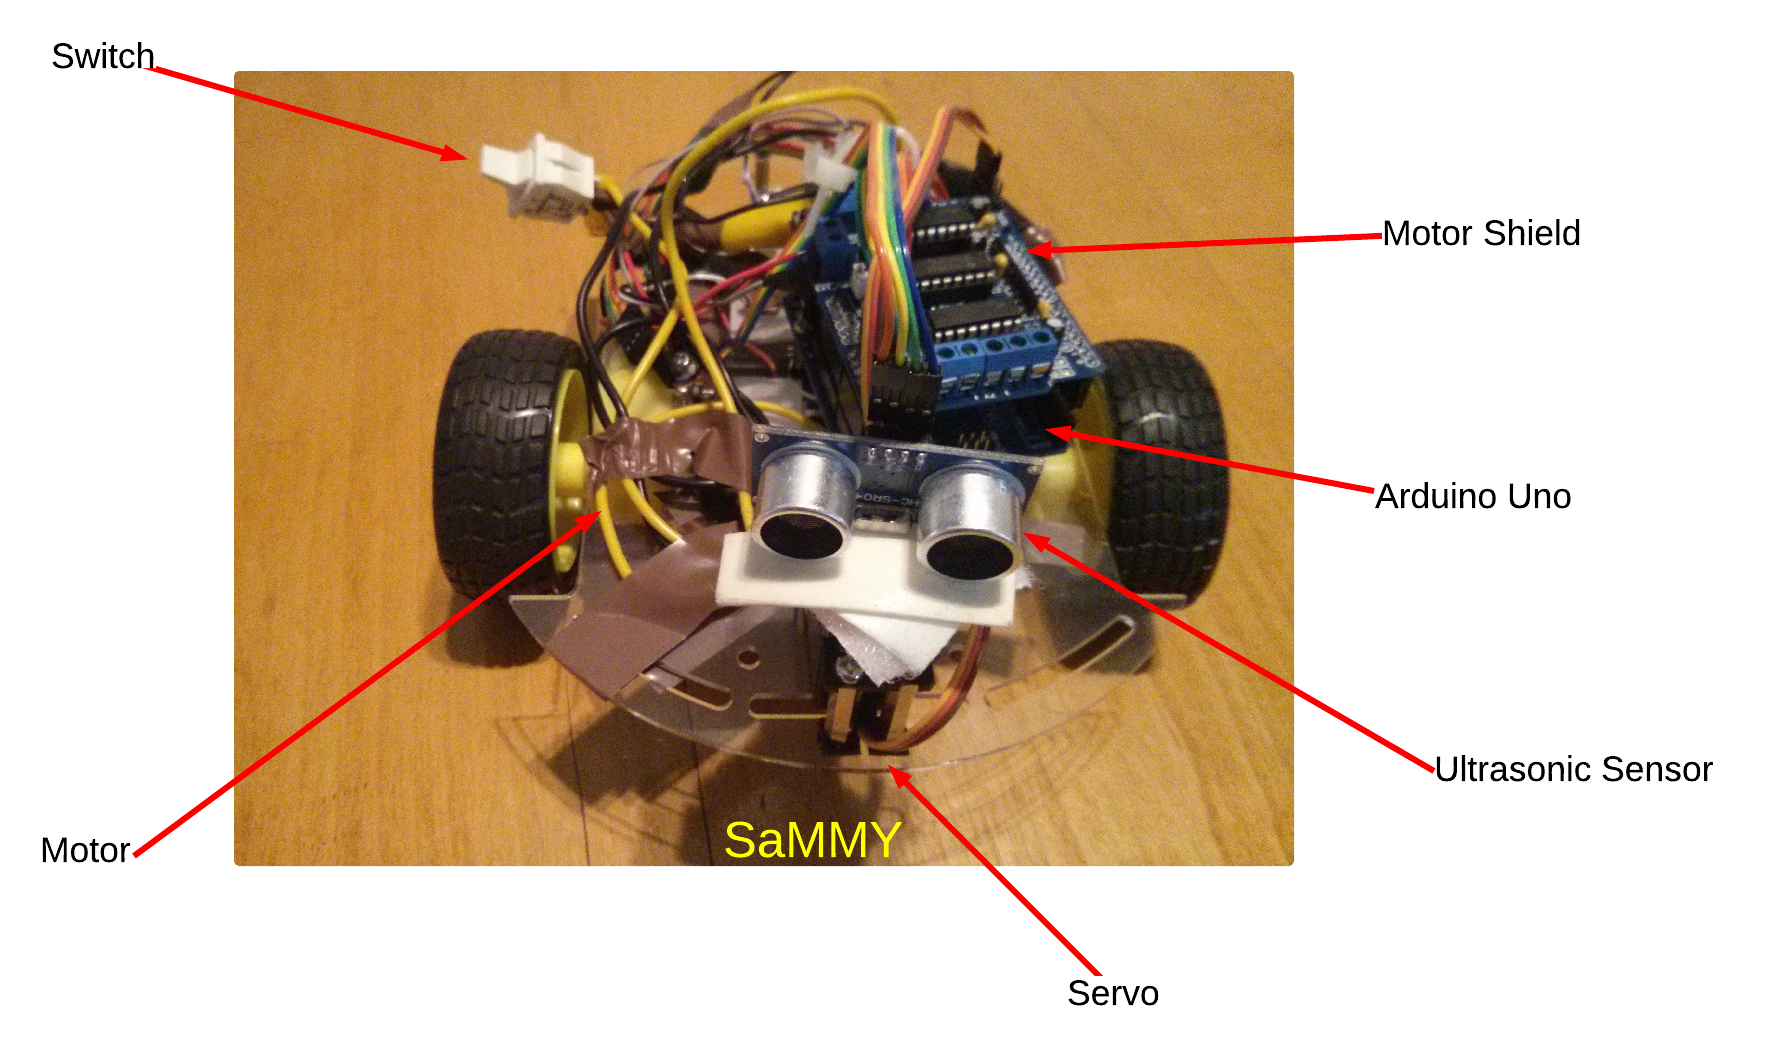
\includegraphics[height=0.57\textwidth]{images/bot_diagram.png}
	\caption{Block Diagram of Control System}
		\label{diagram}
	\end{figure}

	\begin {table}[h]
	\begin {center} 
	%\vspace{15pt}
	
	\begin{tabular}{||l|c|c||}\hline
	%\multicolumn{3}{ |c| }{\textbf{Component List}} \\\hline	
		\textbf{Part Name}	&	\textbf{Function}	&	\textbf{Details}		\\\hline
		1. Motor 		&	Drives wheels				&	N/A 		\\\hline
		2. RadioShack\textsuperscript{\textregistered} Standard Servo		&	180\degree rotation 		&	\url{http://shack.net/Ty2VB4} 		\\\hline
		3. Ultrasonic Ranging Module HC-SR04		&	Object detection	&	\url{http://bit.ly/1lhqwjI}	 	\\\hline
		4. Arduino Uno		&	Microcontroller Board			&	\url{http://bit.ly/1gBB1NG} 		\\\hline
		5.	L293D Motor Driver Shield	&	Controls motors &	\url{http://bit.ly/1uILISF}	\\\hline
		6. Switch	&	On/Off power button &	N/A	\\\hline
		7. Batteries (not pictured) & 	9V AA External Power & 	For Arduino/motors/servo \\\hline

		
	\end{tabular}
		\caption {Hardware Components List} \label{components}
	\end{center}
	\end{table} 		
	
Assembling the kit took a fair amount of time.  We added a switch, soldered pins onto the motor shield for the sonar sensor, added the motor shield, changed the weight a few different times, and taped the battery holder to ensure the batteries wouldn't get displaced. 


\section{Robot Control}

\subsection{Functions}
The software portion was written in the \textbf{Arduino} IDE, and we modified some of the existing libraries.  The main functions for our project are listed in Table \ref{functions}.  
	\begin {table}[h!]
	\begin {center} 
	\vspace{15pt}
	
	\begin{tabular}{||c|c|l||}\hline	
		\textbf{Component}	&	\textbf{Function}	&	\textbf{Details}		\\\hline
		\multirow{5}{*}{Motor}
						&	Drive Forward		&	Both wheels moving forward at predefined speed 		\\
						&	Drive Backward		&	Both wheels moving backward at predefined speed 		\\
						&	Rotate Left/Right	&	Both wheels spin for ``in-place'' turn of 90\degree	 	\\
						&	Veer Left/Right		&	Only outside wheel turns and vehicle does not stop\\
						&	U-Turn				&	Backs up then turns 180\degree		\\
						&	Coolness			&	After certain time, bot does various spins	\\\hline
		\multirow{2}{*}{Sonar + Servo}
						&	Look Forward		&	Scans a 40\degree range in front while moving forward \\
					&	Look Left/Right		&	Scans 90\degree left/right to determine next turn \\\hline


		
	\end{tabular}
		\caption {Robot Functions} \label{functions}
	\end{center}
	\end{table} 	

%scan partial left and right when driving forward, get average
%scan fully left and right, get average
%

After initializing our components, the software ran an infinite loop which scans for objects and makes decisions on which direction to go.  The main control flow is seen in listing \ref{loop} below.

\vspace{12pt}

 \begin{lstlisting}[caption=Control Loop, label=loop]		
  void loop() {
    if (scanClear())  // If clear to go forward
    {
      drive_forward();
    }
    else              // if path is blocked
    {
      freewheel();    // stop
      lookLeft();
      int distanceLeft = getAverageDistance();

      lookRight();
      int distanceRight = getAverageDistance();
      
      // re-center the ultrasonic
      servo_position(CENTER);

      // go the least obstructed way
      if (distanceLeft > distanceRight && distanceLeft > dangerThreshold)       
      {
        drive_backward();
        delay(400);
        rotate_left();
      }
      else if (distanceRight > distanceLeft && distanceRight > dangerThreshold) 
      {
        drive_backward();
        delay(400);
        rotate_right();
      }
      else 		// equally blocked or less than danger threshold left or right
      {
        freewheel();
        delay(20);
        drive_backward();
        delay(500);
        u_turn();
      }   
    } 
  }  
  }
  \end{lstlisting}

%TODO flow diagrams, mockups of components, block diagram (edit battery holder)

\subsection{Algorithm}

%Talk about the specific algorithms, referring to the figures.
%Mention victory dance
%TODO Do we need this since the code above explains this? -- YES because this is the way Roy wants reports .. trust me
%TODO Mention intervals of 10 degrees and how they are averaged

	\begin{figure}[h]\centering
	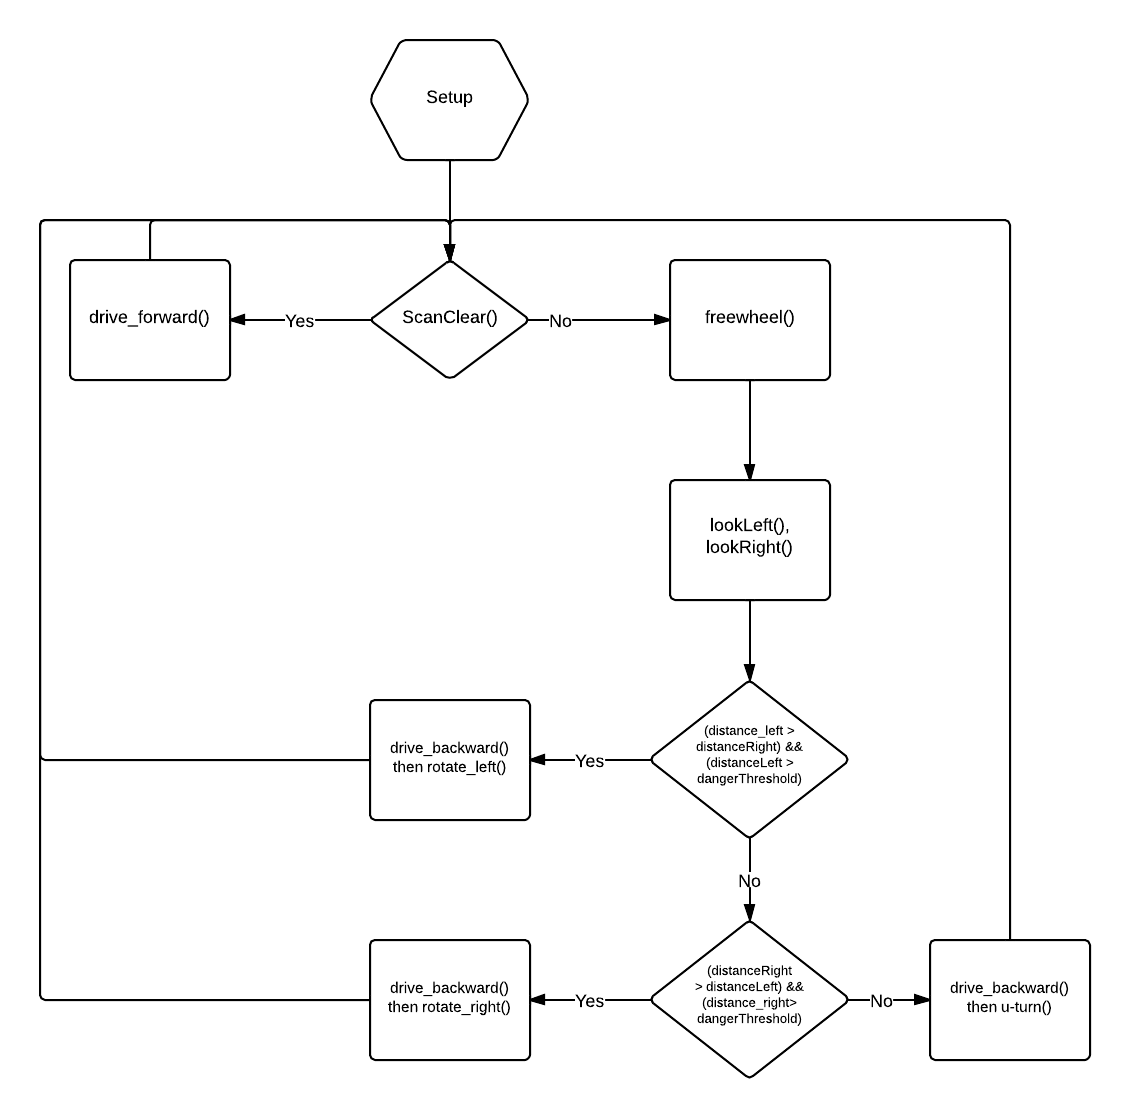
\includegraphics[height=0.85\textwidth]{images/main.png}
	\caption{Main Loop Flowchart}
		\label{main}
	\end{figure}


	\begin{figure}[h]\centering
	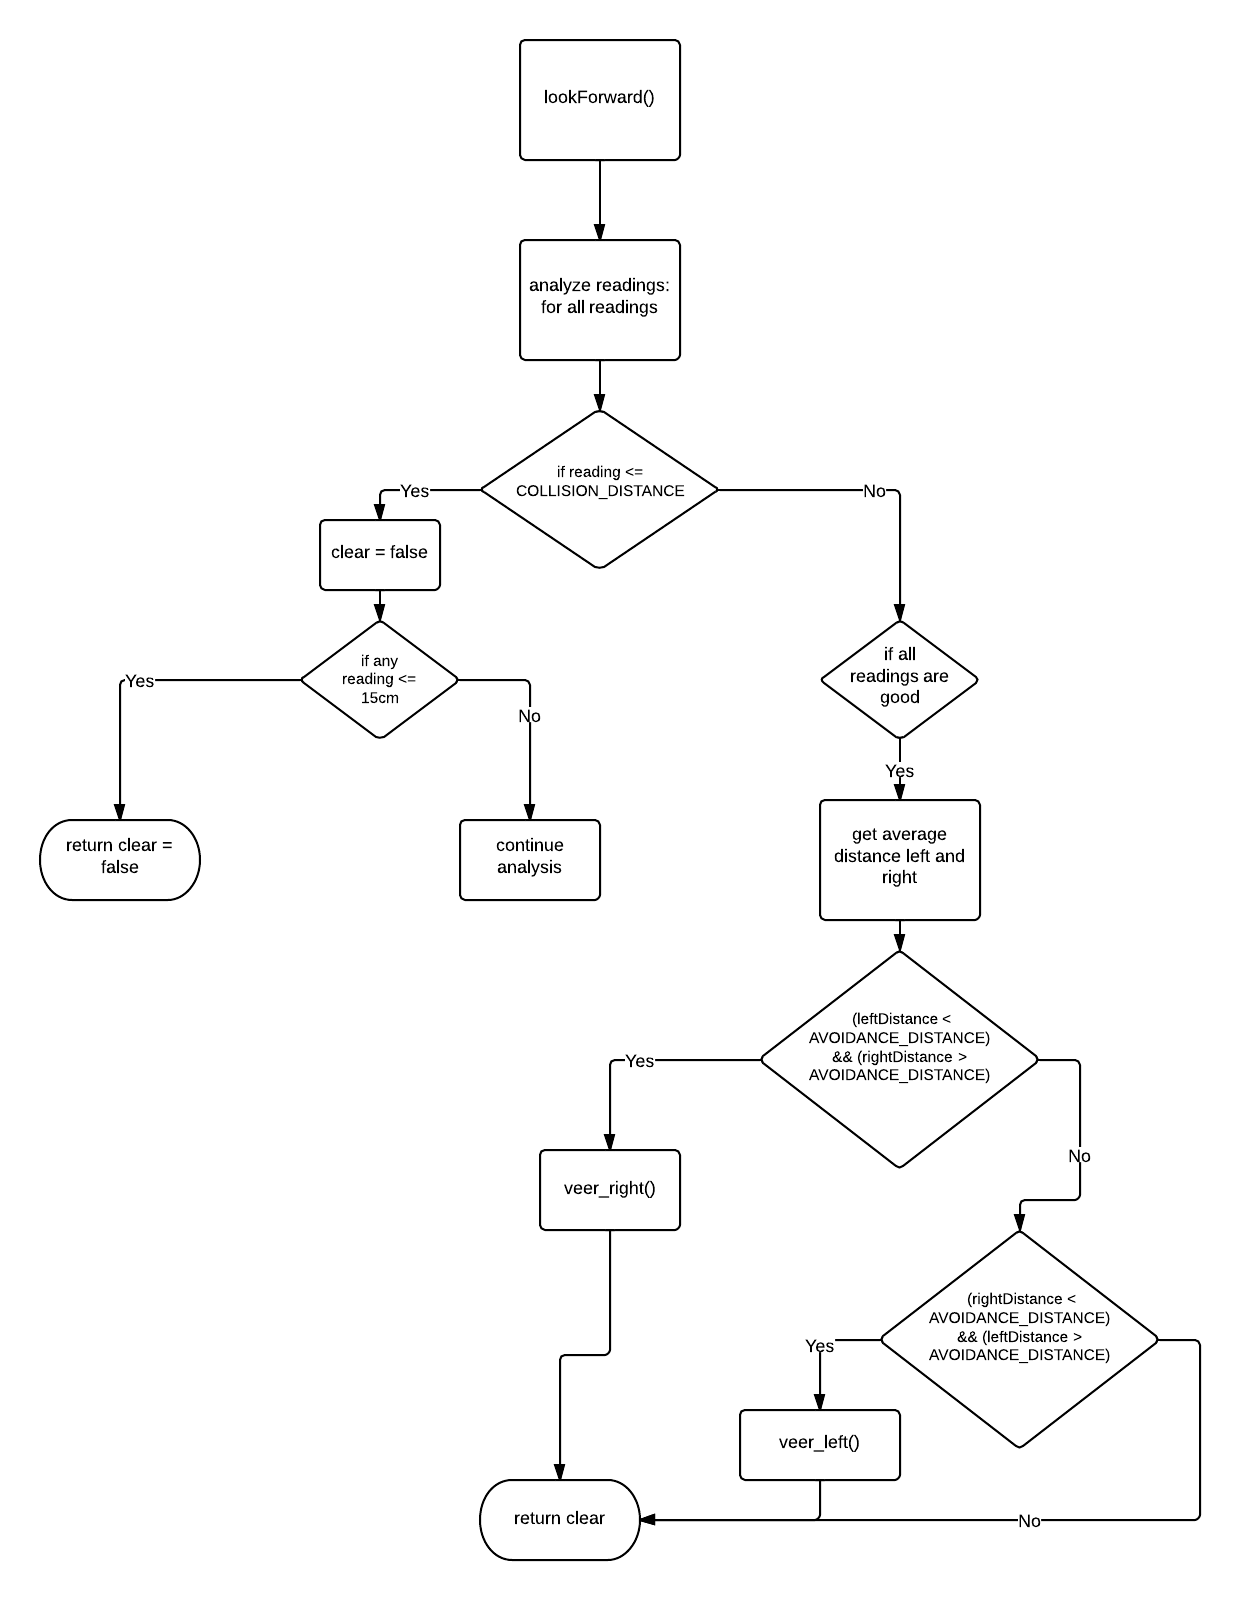
\includegraphics[height=0.85\textwidth]{images/scan_clear.png}
	\caption{Scan Flowchart}
		\label{scan}
	\end{figure}
\par
This program controls the servo and protecto robot car. The bot has one important task ``avoid obstacles''. The main function ``loop'' is called after the setup is done. In that function, there is a counter that will tell the bot when to do its ``victory dance''. If it is not the time for dancing, the scanClear() function is called. If the return value is TRUE (i.e. clear), the bot drives forward. Otherwise, it stops then calls ``lookLeft()'' and ``lookRight()'' and gets the average distances to its left and right. If the distanceLeft is greater than the distanceRight and greater than the ``dangerThreshold'' then the bot backs up and rotates left. Else if the distanceRight is greater than the distanceLeft and greater than the ``dangerThreshold'' then the bot backs up and rotates right. Otherwise, it is blocked on both sides. Therefore, it backs up and makes a u-turn.

%  Note: the "rotate" functions use two wheels one forward and one backward to make a quick move. The "veer" functions only use one wheel to do a slow veer movement.
% 
However, if it is the time to dance, then the ``coolness()'' function is called and the bot performs its victory dance.

The scanClear() function calls the lookForward() function and analyzes the data that is returned by it. It goes through all the readings and checks if any of the distances returned is below the COLLISION\_DISTANCE. If it is, then it sets the clear flag to FALSE and continues the analysis.

However, if a distance is below the COLLISION\_DISTANCE and below the EMERGENCY\_DISTANCE then it directly returns FALSE and exits the function so that the correct reaction takes place. Otherwise, it finishes the analysis and sets the clear flag to TRUE. Then, it checks the average distance on the left and right of the data gathered by looking forward.

If the leftDistance is less than the AVOIDANCE\_DISTANCE and the rightDistance is greater than the AVOIDANCE\_DISTANCE, then the bot veers right.
Else if the rightDistance is less than the AVOIDANCE\_DISTANCE and the leftDistance is greater than the AVOIDANCE\_DISTANCE, then the bot veers left.

The look functions set up the angles and call the scan() function.
 
The scan() function actually performs the scans at each angle by sending a sonar "ping" and waiting for the return signal to measure the distance. Sometime the sonar returns very low values that are not correct which would make the bot stop even if there is no obstacle. To avoid that, in the scan function, if the returned distance is below the EMERGENCY\_DISTANCE then the bot sends another ping. If that newly measured distance is still below the EMERGENCY\_DISTANCE, then it re-centers the sonar and stops scanning so that the necessary reaction takes place as soon as possible.

Acknowledgement: this algorithm is based on the functions and sample sketch provided by oddWires with the purchase of the oddWires Arduino Kit.
                 We used the idea behind the code but we repurposed the functions and used our own algorithms which basically made the bot behave 
                 better in emergency situations and avoid obstacles in a smoother way. 




\section{Conclusion}
\texttt{Servo and Protecto} was quite fun for us to build and was certainly the biggest ``crowd pleaser'' out of all the projects we've made.  The assembly perhaps took the least amount of time, although we did face problems with a few of the parts not being built correctly (mainly the battery holder and motor plate mount).  Fixing the power problems was the most frustrating part of the project, but once we finished everything, the final product was quite rewarding.  We both spent equal times on all the different aspects of this project.  Currently, SaMMY performs quite well, even if he does run into walls occasionally.  This is caused by veering, which was a tough issue to fix. Listed below are some of the challenges we faced.
	
	\subsection{Challenges}
		
		\begin{itemize}				
		\item \textbf{Power Issues}: After the initial assembly, we were not able to properly move the servo and control the motors.  Our initial thought was inadequate power, but the correspondent we communicated with ensured us that it could run perfectly fine on 6V of AA batteries.  Even after upping the voltage we saw problems, which were due to the power demands of our servo.  After increasing the power to 9V of AA batteries the problem diminished.
		\item \textbf{Motor control}: The motors we received are not precise enough to deliver equal power on both sides.  This caused inevitable veering of the robot.  We were able to use our own veering function to correct a lot of this, but were not able to control the bot perfectly.
		\item \textbf{CMUcam}: We were able to calibrate and test the CMUcam, which was intended for color detection.  However, communicating the frames from the camera to the Arduino proved difficult.  Even the example code would not work on our device. We were not able to solve the communication error before the project was due.
		\item \textbf{Erroneous Sonar Readings}: Occasionally the ultrasonic sensor picked up erroneous values that would usually be below 10cm (possibly due to ghost echoes).  This cause the robot to stop immediately.  We adjusted this by filtering out the first ping that it received below 10cm.
		\end{itemize}

\subsection{Future Additions}
The Arduino platform and components in this project provide a large amount of functionality.  Because of this, the amount of improvements is virtually limitless.  Our goals in the future could involve adding:
		\begin{itemize}				
		\item \textbf{Battery Pack}: Buying a powerful, rechargeable battery pack would save money, improve performance and decrease hassle.
		\item \textbf{External Apparatus}: We initially wanted to attach a simple device that could be triggered based on certain events.  While launching or shooting an object would have been interesting, in most cases this would require PID algorithms, which would involve sufficiently more work and tuning.
		\item \textbf{Color Detection}: One of our original ideas (and part of the reason for the name \textbf{Servo and Protecto}) was to use color detection to differentiate between ``friends'' and ``enemies''.  There would be certain objects that the robot would purposely avoid, and others that it would just run over.
		\item \textbf{Infrared}: Infrared sensors can be used to detect edges, and they could also be used as an external controller/remote.
		\item \textbf{Object Following}: The sonar and/or color detector could be used to follow an object instead of avoid them.  This would be useful when if we attached a physical arm or apparatus of some sort.
		\end{itemize}

\section{References}
%TODO
\textbf{Oddwires} Robot Kit:  \url{http://bit.ly/TysmCv}
Arduino Libraries
Pictures
\end{document}
%references
%-oddwires
%-arduino
